% Created by tikzDevice version 0.12.3.1 on 2021-05-25 15:52:59
% !TEX encoding = UTF-8 Unicode
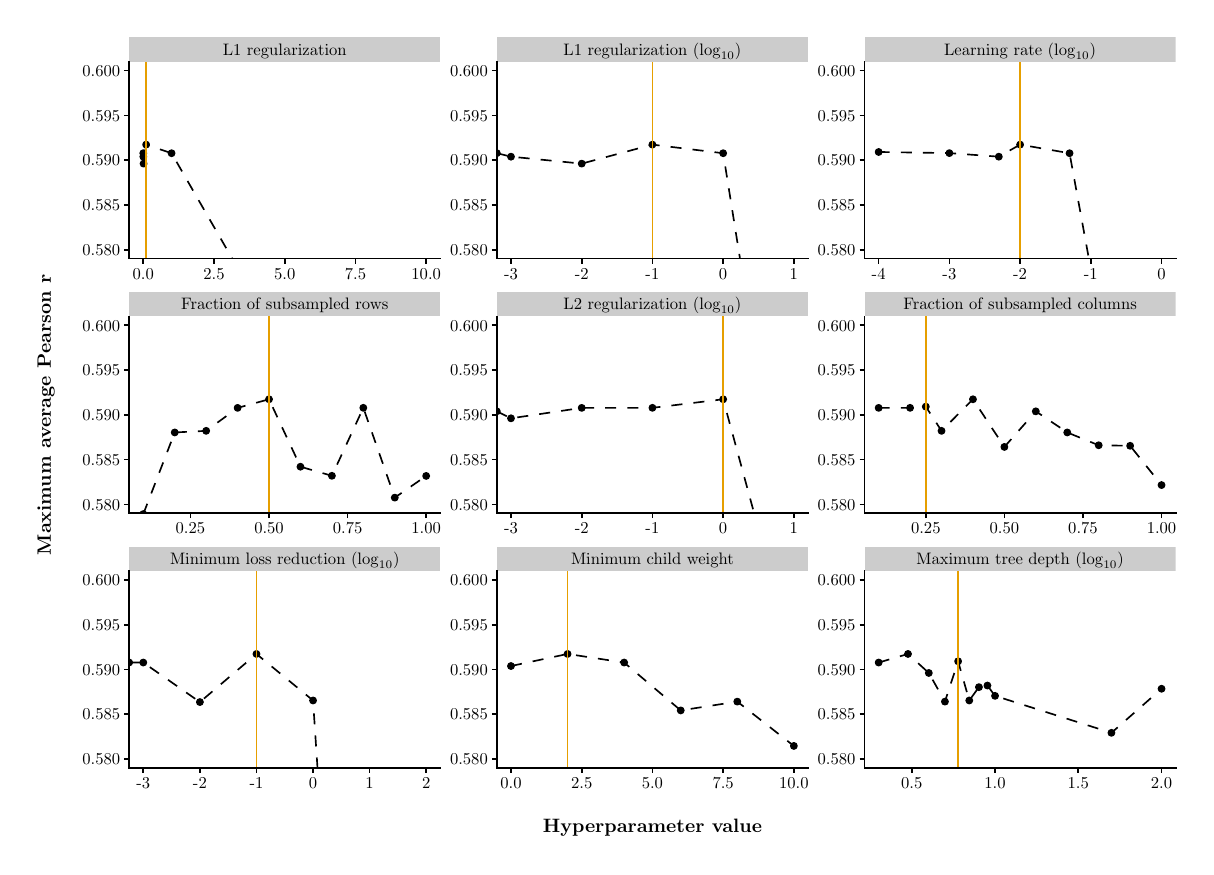
\begin{tikzpicture}[x=1pt,y=1pt]
\definecolor{fillColor}{RGB}{255,255,255}
\path[use as bounding box,fill=fillColor,fill opacity=0.00] (0,0) rectangle (418.34,295.82);
\begin{scope}
\path[clip] ( 36.67,212.35) rectangle (149.11,283.52);
\definecolor{drawColor}{RGB}{0,0,0}
\definecolor{fillColor}{RGB}{0,0,0}

\path[draw=drawColor,line width= 0.4pt,line join=round,line cap=round,fill=fillColor] ( 41.78,250.47) circle (  1.21);

\path[draw=drawColor,line width= 0.4pt,line join=round,line cap=round,fill=fillColor] ( 41.79,249.20) circle (  1.21);

\path[draw=drawColor,line width= 0.4pt,line join=round,line cap=round,fill=fillColor] ( 41.88,246.69) circle (  1.21);

\path[draw=drawColor,line width= 0.4pt,line join=round,line cap=round,fill=fillColor] ( 42.80,253.56) circle (  1.21);

\path[draw=drawColor,line width= 0.4pt,line join=round,line cap=round,fill=fillColor] ( 52.00,250.45) circle (  1.21);

\path[draw=drawColor,line width= 0.4pt,line join=round,line cap=round,fill=fillColor] (144.00, 90.55) circle (  1.21);

\path[draw=drawColor,line width= 0.6pt,dash pattern=on 4pt off 4pt ,line join=round] ( 41.78,250.47) --
	( 41.79,249.20) --
	( 41.88,246.69) --
	( 42.80,253.56) --
	( 52.00,250.45) --
	(144.00, 90.55);
\definecolor{drawColor}{RGB}{230,159,0}

\path[draw=drawColor,line width= 0.6pt,line join=round] ( 42.80,212.35) -- ( 42.80,283.52);
\end{scope}
\begin{scope}
\path[clip] ( 36.67,120.33) rectangle (149.11,191.50);
\definecolor{drawColor}{RGB}{0,0,0}
\definecolor{fillColor}{RGB}{0,0,0}

\path[draw=drawColor,line width= 0.4pt,line join=round,line cap=round,fill=fillColor] ( 41.78,120.05) circle (  1.21);

\path[draw=drawColor,line width= 0.4pt,line join=round,line cap=round,fill=fillColor] ( 53.14,149.55) circle (  1.21);

\path[draw=drawColor,line width= 0.4pt,line join=round,line cap=round,fill=fillColor] ( 64.50,150.13) circle (  1.21);

\path[draw=drawColor,line width= 0.4pt,line join=round,line cap=round,fill=fillColor] ( 75.86,158.43) circle (  1.21);

\path[draw=drawColor,line width= 0.4pt,line join=round,line cap=round,fill=fillColor] ( 87.21,161.54) circle (  1.21);

\path[draw=drawColor,line width= 0.4pt,line join=round,line cap=round,fill=fillColor] ( 98.57,137.17) circle (  1.21);

\path[draw=drawColor,line width= 0.4pt,line join=round,line cap=round,fill=fillColor] (109.93,133.89) circle (  1.21);

\path[draw=drawColor,line width= 0.4pt,line join=round,line cap=round,fill=fillColor] (121.29,158.45) circle (  1.21);

\path[draw=drawColor,line width= 0.4pt,line join=round,line cap=round,fill=fillColor] (132.65,126.00) circle (  1.21);

\path[draw=drawColor,line width= 0.4pt,line join=round,line cap=round,fill=fillColor] (144.00,133.84) circle (  1.21);

\path[draw=drawColor,line width= 0.6pt,dash pattern=on 4pt off 4pt ,line join=round] ( 41.78,120.05) --
	( 53.14,149.55) --
	( 64.50,150.13) --
	( 75.86,158.43) --
	( 87.21,161.54) --
	( 98.57,137.17) --
	(109.93,133.89) --
	(121.29,158.45) --
	(132.65,126.00) --
	(144.00,133.84);
\definecolor{drawColor}{RGB}{230,159,0}

\path[draw=drawColor,line width= 0.6pt,line join=round] ( 87.21,120.33) -- ( 87.21,191.50);
\end{scope}
\begin{scope}
\path[clip] ( 36.67, 28.30) rectangle (149.11, 99.48);
\definecolor{drawColor}{RGB}{0,0,0}
\definecolor{fillColor}{RGB}{0,0,0}

\path[draw=drawColor,line width= 0.4pt,line join=round,line cap=round,fill=fillColor] ( 36.67, 66.43) circle (  1.21);

\path[draw=drawColor,line width= 0.4pt,line join=round,line cap=round,fill=fillColor] ( 41.78, 66.41) circle (  1.21);

\path[draw=drawColor,line width= 0.4pt,line join=round,line cap=round,fill=fillColor] ( 62.23, 52.13) circle (  1.21);

\path[draw=drawColor,line width= 0.4pt,line join=round,line cap=round,fill=fillColor] ( 82.67, 69.51) circle (  1.21);

\path[draw=drawColor,line width= 0.4pt,line join=round,line cap=round,fill=fillColor] (103.12, 52.70) circle (  1.21);

\path[draw=drawColor,line width= 0.4pt,line join=round,line cap=round,fill=fillColor] (123.56,-257.84) circle (  1.21);

\path[draw=drawColor,line width= 0.4pt,line join=round,line cap=round,fill=fillColor] (144.00,-1280.79) circle (  1.21);

\path[draw=drawColor,line width= 0.6pt,dash pattern=on 4pt off 4pt ,line join=round] ( 36.67, 66.43) --
	( 41.78, 66.41) --
	( 62.23, 52.13) --
	( 82.67, 69.51) --
	(103.12, 52.70) --
	(123.56,-257.84) --
	(144.00,-1280.79);
\definecolor{drawColor}{RGB}{230,159,0}

\path[draw=drawColor,line width= 0.6pt,line join=round] ( 82.67, 28.30) -- ( 82.67, 99.48);
\end{scope}
\begin{scope}
\path[clip] (169.53,212.35) rectangle (281.98,283.52);
\definecolor{drawColor}{RGB}{0,0,0}
\definecolor{fillColor}{RGB}{0,0,0}

\path[draw=drawColor,line width= 0.4pt,line join=round,line cap=round,fill=fillColor] (169.53,250.47) circle (  1.21);

\path[draw=drawColor,line width= 0.4pt,line join=round,line cap=round,fill=fillColor] (174.64,249.20) circle (  1.21);

\path[draw=drawColor,line width= 0.4pt,line join=round,line cap=round,fill=fillColor] (200.20,246.69) circle (  1.21);

\path[draw=drawColor,line width= 0.4pt,line join=round,line cap=round,fill=fillColor] (225.75,253.56) circle (  1.21);

\path[draw=drawColor,line width= 0.4pt,line join=round,line cap=round,fill=fillColor] (251.31,250.45) circle (  1.21);

\path[draw=drawColor,line width= 0.4pt,line join=round,line cap=round,fill=fillColor] (276.86, 90.55) circle (  1.21);

\path[draw=drawColor,line width= 0.6pt,dash pattern=on 4pt off 4pt ,line join=round] (169.53,250.47) --
	(174.64,249.20) --
	(200.20,246.69) --
	(225.75,253.56) --
	(251.31,250.45) --
	(276.86, 90.55);
\definecolor{drawColor}{RGB}{230,159,0}

\path[draw=drawColor,line width= 0.6pt,line join=round] (225.75,212.35) -- (225.75,283.52);
\end{scope}
\begin{scope}
\path[clip] (169.53,120.33) rectangle (281.98,191.50);
\definecolor{drawColor}{RGB}{0,0,0}
\definecolor{fillColor}{RGB}{0,0,0}

\path[draw=drawColor,line width= 0.4pt,line join=round,line cap=round,fill=fillColor] (169.53,157.18) circle (  1.21);

\path[draw=drawColor,line width= 0.4pt,line join=round,line cap=round,fill=fillColor] (174.64,154.66) circle (  1.21);

\path[draw=drawColor,line width= 0.4pt,line join=round,line cap=round,fill=fillColor] (200.20,158.43) circle (  1.21);

\path[draw=drawColor,line width= 0.4pt,line join=round,line cap=round,fill=fillColor] (225.75,158.45) circle (  1.21);

\path[draw=drawColor,line width= 0.4pt,line join=round,line cap=round,fill=fillColor] (251.31,161.54) circle (  1.21);

\path[draw=drawColor,line width= 0.4pt,line join=round,line cap=round,fill=fillColor] (266.69,104.97) circle (  1.21);

\path[draw=drawColor,line width= 0.4pt,line join=round,line cap=round,fill=fillColor] (276.86,105.81) circle (  1.21);

\path[draw=drawColor,line width= 0.6pt,dash pattern=on 4pt off 4pt ,line join=round] (169.53,157.18) --
	(174.64,154.66) --
	(200.20,158.43) --
	(225.75,158.45) --
	(251.31,161.54) --
	(266.69,104.97) --
	(276.86,105.81);
\definecolor{drawColor}{RGB}{230,159,0}

\path[draw=drawColor,line width= 0.6pt,line join=round] (251.31,120.33) -- (251.31,191.50);
\end{scope}
\begin{scope}
\path[clip] (169.53, 28.30) rectangle (281.98, 99.48);
\definecolor{drawColor}{RGB}{0,0,0}
\definecolor{fillColor}{RGB}{0,0,0}

\path[draw=drawColor,line width= 0.4pt,line join=round,line cap=round,fill=fillColor] (174.64, 65.15) circle (  1.21);

\path[draw=drawColor,line width= 0.4pt,line join=round,line cap=round,fill=fillColor] (195.09, 69.51) circle (  1.21);

\path[draw=drawColor,line width= 0.4pt,line join=round,line cap=round,fill=fillColor] (215.53, 66.41) circle (  1.21);

\path[draw=drawColor,line width= 0.4pt,line join=round,line cap=round,fill=fillColor] (235.98, 49.11) circle (  1.21);

\path[draw=drawColor,line width= 0.4pt,line join=round,line cap=round,fill=fillColor] (256.42, 52.29) circle (  1.21);

\path[draw=drawColor,line width= 0.4pt,line join=round,line cap=round,fill=fillColor] (276.86, 36.28) circle (  1.21);

\path[draw=drawColor,line width= 0.6pt,dash pattern=on 4pt off 4pt ,line join=round] (174.64, 65.15) --
	(195.09, 69.51) --
	(215.53, 66.41) --
	(235.98, 49.11) --
	(256.42, 52.29) --
	(276.86, 36.28);
\definecolor{drawColor}{RGB}{230,159,0}

\path[draw=drawColor,line width= 0.6pt,line join=round] (195.09, 28.30) -- (195.09, 99.48);
\end{scope}
\begin{scope}
\path[clip] (302.39,212.35) rectangle (414.84,283.52);
\definecolor{drawColor}{RGB}{0,0,0}
\definecolor{fillColor}{RGB}{0,0,0}

\path[draw=drawColor,line width= 0.4pt,line join=round,line cap=round,fill=fillColor] (307.50,250.90) circle (  1.21);

\path[draw=drawColor,line width= 0.4pt,line join=round,line cap=round,fill=fillColor] (333.06,250.49) circle (  1.21);

\path[draw=drawColor,line width= 0.4pt,line join=round,line cap=round,fill=fillColor] (350.92,249.20) circle (  1.21);

\path[draw=drawColor,line width= 0.4pt,line join=round,line cap=round,fill=fillColor] (358.61,253.56) circle (  1.21);

\path[draw=drawColor,line width= 0.4pt,line join=round,line cap=round,fill=fillColor] (376.48,250.45) circle (  1.21);

\path[draw=drawColor,line width= 0.4pt,line join=round,line cap=round,fill=fillColor] (384.17,208.48) circle (  1.21);

\path[draw=drawColor,line width= 0.4pt,line join=round,line cap=round,fill=fillColor] (402.03, 73.04) circle (  1.21);

\path[draw=drawColor,line width= 0.4pt,line join=round,line cap=round,fill=fillColor] (409.72,-308.77) circle (  1.21);

\path[draw=drawColor,line width= 0.6pt,dash pattern=on 4pt off 4pt ,line join=round] (307.50,250.90) --
	(333.06,250.49) --
	(350.92,249.20) --
	(358.61,253.56) --
	(376.48,250.45) --
	(384.17,208.48) --
	(402.03, 73.04) --
	(409.72,-308.77);
\definecolor{drawColor}{RGB}{230,159,0}

\path[draw=drawColor,line width= 0.6pt,line join=round] (358.61,212.35) -- (358.61,283.52);
\end{scope}
\begin{scope}
\path[clip] (302.39,120.33) rectangle (414.84,191.50);
\definecolor{drawColor}{RGB}{0,0,0}
\definecolor{fillColor}{RGB}{0,0,0}

\path[draw=drawColor,line width= 0.4pt,line join=round,line cap=round,fill=fillColor] (307.50,158.43) circle (  1.21);

\path[draw=drawColor,line width= 0.4pt,line join=round,line cap=round,fill=fillColor] (318.86,158.45) circle (  1.21);

\path[draw=drawColor,line width= 0.4pt,line join=round,line cap=round,fill=fillColor] (324.54,158.88) circle (  1.21);

\path[draw=drawColor,line width= 0.4pt,line join=round,line cap=round,fill=fillColor] (330.22,150.13) circle (  1.21);

\path[draw=drawColor,line width= 0.4pt,line join=round,line cap=round,fill=fillColor] (341.58,161.54) circle (  1.21);

\path[draw=drawColor,line width= 0.4pt,line join=round,line cap=round,fill=fillColor] (352.93,144.32) circle (  1.21);

\path[draw=drawColor,line width= 0.4pt,line join=round,line cap=round,fill=fillColor] (364.29,157.18) circle (  1.21);

\path[draw=drawColor,line width= 0.4pt,line join=round,line cap=round,fill=fillColor] (375.65,149.55) circle (  1.21);

\path[draw=drawColor,line width= 0.4pt,line join=round,line cap=round,fill=fillColor] (387.01,144.92) circle (  1.21);

\path[draw=drawColor,line width= 0.4pt,line join=round,line cap=round,fill=fillColor] (398.37,144.73) circle (  1.21);

\path[draw=drawColor,line width= 0.4pt,line join=round,line cap=round,fill=fillColor] (409.72,130.54) circle (  1.21);

\path[draw=drawColor,line width= 0.6pt,dash pattern=on 4pt off 4pt ,line join=round] (307.50,158.43) --
	(318.86,158.45) --
	(324.54,158.88) --
	(330.22,150.13) --
	(341.58,161.54) --
	(352.93,144.32) --
	(364.29,157.18) --
	(375.65,149.55) --
	(387.01,144.92) --
	(398.37,144.73) --
	(409.72,130.54);
\definecolor{drawColor}{RGB}{230,159,0}

\path[draw=drawColor,line width= 0.6pt,line join=round] (324.54,120.33) -- (324.54,191.50);
\end{scope}
\begin{scope}
\path[clip] (302.39, 28.30) rectangle (414.84, 99.48);
\definecolor{drawColor}{RGB}{0,0,0}
\definecolor{fillColor}{RGB}{0,0,0}

\path[draw=drawColor,line width= 0.4pt,line join=round,line cap=round,fill=fillColor] (307.50, 66.41) circle (  1.21);

\path[draw=drawColor,line width= 0.4pt,line join=round,line cap=round,fill=fillColor] (318.10, 69.51) circle (  1.21);

\path[draw=drawColor,line width= 0.4pt,line join=round,line cap=round,fill=fillColor] (325.62, 62.64) circle (  1.21);

\path[draw=drawColor,line width= 0.4pt,line join=round,line cap=round,fill=fillColor] (331.45, 52.29) circle (  1.21);

\path[draw=drawColor,line width= 0.4pt,line join=round,line cap=round,fill=fillColor] (336.21, 66.86) circle (  1.21);

\path[draw=drawColor,line width= 0.4pt,line join=round,line cap=round,fill=fillColor] (340.24, 52.70) circle (  1.21);

\path[draw=drawColor,line width= 0.4pt,line join=round,line cap=round,fill=fillColor] (343.73, 57.52) circle (  1.21);

\path[draw=drawColor,line width= 0.4pt,line join=round,line cap=round,fill=fillColor] (346.80, 58.10) circle (  1.21);

\path[draw=drawColor,line width= 0.4pt,line join=round,line cap=round,fill=fillColor] (349.56, 54.37) circle (  1.21);

\path[draw=drawColor,line width= 0.4pt,line join=round,line cap=round,fill=fillColor] (391.61, 41.01) circle (  1.21);

\path[draw=drawColor,line width= 0.4pt,line join=round,line cap=round,fill=fillColor] (409.72, 56.94) circle (  1.21);

\path[draw=drawColor,line width= 0.6pt,dash pattern=on 4pt off 4pt ,line join=round] (307.50, 66.41) --
	(318.10, 69.51) --
	(325.62, 62.64) --
	(331.45, 52.29) --
	(336.21, 66.86) --
	(340.24, 52.70) --
	(343.73, 57.52) --
	(346.80, 58.10) --
	(349.56, 54.37) --
	(391.61, 41.01) --
	(409.72, 56.94);
\definecolor{drawColor}{RGB}{230,159,0}

\path[draw=drawColor,line width= 0.6pt,line join=round] (336.21, 28.30) -- (336.21, 99.48);
\end{scope}
\begin{scope}
\path[clip] ( 36.67, 99.48) rectangle (149.11,108.28);
\definecolor{fillColor}{gray}{0.80}

\path[fill=fillColor] ( 36.67, 99.48) rectangle (149.11,108.28);
\definecolor{drawColor}{RGB}{0,0,0}

\node[text=drawColor,anchor=base,inner sep=0pt, outer sep=0pt, scale=  0.60] at ( 92.89,101.81) {Minimum loss reduction ($\log_{10}$)};
\end{scope}
\begin{scope}
\path[clip] (169.53, 99.48) rectangle (281.98,108.28);
\definecolor{fillColor}{gray}{0.80}

\path[fill=fillColor] (169.53, 99.48) rectangle (281.98,108.28);
\definecolor{drawColor}{RGB}{0,0,0}

\node[text=drawColor,anchor=base,inner sep=0pt, outer sep=0pt, scale=  0.60] at (225.75,101.81) {Minimum child weight};
\end{scope}
\begin{scope}
\path[clip] (302.39, 99.48) rectangle (414.84,108.28);
\definecolor{fillColor}{gray}{0.80}

\path[fill=fillColor] (302.39, 99.48) rectangle (414.84,108.28);
\definecolor{drawColor}{RGB}{0,0,0}

\node[text=drawColor,anchor=base,inner sep=0pt, outer sep=0pt, scale=  0.60] at (358.61,101.81) {Maximum tree depth ($\log_{10}$)};
\end{scope}
\begin{scope}
\path[clip] ( 36.67,191.50) rectangle (149.11,200.30);
\definecolor{fillColor}{gray}{0.80}

\path[fill=fillColor] ( 36.67,191.50) rectangle (149.11,200.30);
\definecolor{drawColor}{RGB}{0,0,0}

\node[text=drawColor,anchor=base,inner sep=0pt, outer sep=0pt, scale=  0.60] at ( 92.89,193.83) {Fraction of subsampled rows};
\end{scope}
\begin{scope}
\path[clip] (169.53,191.50) rectangle (281.98,200.30);
\definecolor{fillColor}{gray}{0.80}

\path[fill=fillColor] (169.53,191.50) rectangle (281.98,200.30);
\definecolor{drawColor}{RGB}{0,0,0}

\node[text=drawColor,anchor=base,inner sep=0pt, outer sep=0pt, scale=  0.60] at (225.75,193.83) {L2 regularization ($\log_{10}$)};
\end{scope}
\begin{scope}
\path[clip] (302.39,191.50) rectangle (414.84,200.30);
\definecolor{fillColor}{gray}{0.80}

\path[fill=fillColor] (302.39,191.50) rectangle (414.84,200.30);
\definecolor{drawColor}{RGB}{0,0,0}

\node[text=drawColor,anchor=base,inner sep=0pt, outer sep=0pt, scale=  0.60] at (358.61,193.83) {Fraction of subsampled columns};
\end{scope}
\begin{scope}
\path[clip] ( 36.67,283.52) rectangle (149.11,292.32);
\definecolor{fillColor}{gray}{0.80}

\path[fill=fillColor] ( 36.67,283.52) rectangle (149.11,292.32);
\definecolor{drawColor}{RGB}{0,0,0}

\node[text=drawColor,anchor=base,inner sep=0pt, outer sep=0pt, scale=  0.60] at ( 92.89,285.86) {L1 regularization};
\end{scope}
\begin{scope}
\path[clip] (169.53,283.52) rectangle (281.98,292.32);
\definecolor{fillColor}{gray}{0.80}

\path[fill=fillColor] (169.53,283.52) rectangle (281.98,292.32);
\definecolor{drawColor}{RGB}{0,0,0}

\node[text=drawColor,anchor=base,inner sep=0pt, outer sep=0pt, scale=  0.60] at (225.75,285.86) {L1 regularization ($\log_{10}$)};
\end{scope}
\begin{scope}
\path[clip] (302.39,283.52) rectangle (414.84,292.32);
\definecolor{fillColor}{gray}{0.80}

\path[fill=fillColor] (302.39,283.52) rectangle (414.84,292.32);
\definecolor{drawColor}{RGB}{0,0,0}

\node[text=drawColor,anchor=base,inner sep=0pt, outer sep=0pt, scale=  0.60] at (358.61,285.86) {Learning rate ($\log_{10}$)};
\end{scope}
\begin{scope}
\path[clip] (  0.00,  0.00) rectangle (418.34,295.82);
\definecolor{drawColor}{RGB}{0,0,0}

\path[draw=drawColor,line width= 0.6pt,line join=round,line cap=rect] ( 36.67, 28.30) --
	(149.11, 28.30);
\end{scope}
\begin{scope}
\path[clip] (  0.00,  0.00) rectangle (418.34,295.82);
\definecolor{drawColor}{RGB}{0,0,0}

\path[draw=drawColor,line width= 0.6pt,line join=round] ( 41.78, 26.55) --
	( 41.78, 28.30);

\path[draw=drawColor,line width= 0.6pt,line join=round] ( 62.23, 26.55) --
	( 62.23, 28.30);

\path[draw=drawColor,line width= 0.6pt,line join=round] ( 82.67, 26.55) --
	( 82.67, 28.30);

\path[draw=drawColor,line width= 0.6pt,line join=round] (103.12, 26.55) --
	(103.12, 28.30);

\path[draw=drawColor,line width= 0.6pt,line join=round] (123.56, 26.55) --
	(123.56, 28.30);

\path[draw=drawColor,line width= 0.6pt,line join=round] (144.00, 26.55) --
	(144.00, 28.30);
\end{scope}
\begin{scope}
\path[clip] (  0.00,  0.00) rectangle (418.34,295.82);
\definecolor{drawColor}{RGB}{0,0,0}

\node[text=drawColor,anchor=base,inner sep=0pt, outer sep=0pt, scale=  0.60] at ( 41.78, 20.92) {-3};

\node[text=drawColor,anchor=base,inner sep=0pt, outer sep=0pt, scale=  0.60] at ( 62.23, 20.92) {-2};

\node[text=drawColor,anchor=base,inner sep=0pt, outer sep=0pt, scale=  0.60] at ( 82.67, 20.92) {-1};

\node[text=drawColor,anchor=base,inner sep=0pt, outer sep=0pt, scale=  0.60] at (103.12, 20.92) {0};

\node[text=drawColor,anchor=base,inner sep=0pt, outer sep=0pt, scale=  0.60] at (123.56, 20.92) {1};

\node[text=drawColor,anchor=base,inner sep=0pt, outer sep=0pt, scale=  0.60] at (144.00, 20.92) {2};
\end{scope}
\begin{scope}
\path[clip] (  0.00,  0.00) rectangle (418.34,295.82);
\definecolor{drawColor}{RGB}{0,0,0}

\path[draw=drawColor,line width= 0.6pt,line join=round,line cap=rect] (169.53, 28.30) --
	(281.98, 28.30);
\end{scope}
\begin{scope}
\path[clip] (  0.00,  0.00) rectangle (418.34,295.82);
\definecolor{drawColor}{RGB}{0,0,0}

\path[draw=drawColor,line width= 0.6pt,line join=round] (174.64, 26.55) --
	(174.64, 28.30);

\path[draw=drawColor,line width= 0.6pt,line join=round] (200.20, 26.55) --
	(200.20, 28.30);

\path[draw=drawColor,line width= 0.6pt,line join=round] (225.75, 26.55) --
	(225.75, 28.30);

\path[draw=drawColor,line width= 0.6pt,line join=round] (251.31, 26.55) --
	(251.31, 28.30);

\path[draw=drawColor,line width= 0.6pt,line join=round] (276.86, 26.55) --
	(276.86, 28.30);
\end{scope}
\begin{scope}
\path[clip] (  0.00,  0.00) rectangle (418.34,295.82);
\definecolor{drawColor}{RGB}{0,0,0}

\node[text=drawColor,anchor=base,inner sep=0pt, outer sep=0pt, scale=  0.60] at (174.64, 20.92) {0.0};

\node[text=drawColor,anchor=base,inner sep=0pt, outer sep=0pt, scale=  0.60] at (200.20, 20.92) {2.5};

\node[text=drawColor,anchor=base,inner sep=0pt, outer sep=0pt, scale=  0.60] at (225.75, 20.92) {5.0};

\node[text=drawColor,anchor=base,inner sep=0pt, outer sep=0pt, scale=  0.60] at (251.31, 20.92) {7.5};

\node[text=drawColor,anchor=base,inner sep=0pt, outer sep=0pt, scale=  0.60] at (276.86, 20.92) {10.0};
\end{scope}
\begin{scope}
\path[clip] (  0.00,  0.00) rectangle (418.34,295.82);
\definecolor{drawColor}{RGB}{0,0,0}

\path[draw=drawColor,line width= 0.6pt,line join=round,line cap=rect] (302.39, 28.30) --
	(414.84, 28.30);
\end{scope}
\begin{scope}
\path[clip] (  0.00,  0.00) rectangle (418.34,295.82);
\definecolor{drawColor}{RGB}{0,0,0}

\path[draw=drawColor,line width= 0.6pt,line join=round] (319.47, 26.55) --
	(319.47, 28.30);

\path[draw=drawColor,line width= 0.6pt,line join=round] (349.56, 26.55) --
	(349.56, 28.30);

\path[draw=drawColor,line width= 0.6pt,line join=round] (379.64, 26.55) --
	(379.64, 28.30);

\path[draw=drawColor,line width= 0.6pt,line join=round] (409.72, 26.55) --
	(409.72, 28.30);
\end{scope}
\begin{scope}
\path[clip] (  0.00,  0.00) rectangle (418.34,295.82);
\definecolor{drawColor}{RGB}{0,0,0}

\node[text=drawColor,anchor=base,inner sep=0pt, outer sep=0pt, scale=  0.60] at (319.47, 20.92) {0.5};

\node[text=drawColor,anchor=base,inner sep=0pt, outer sep=0pt, scale=  0.60] at (349.56, 20.92) {1.0};

\node[text=drawColor,anchor=base,inner sep=0pt, outer sep=0pt, scale=  0.60] at (379.64, 20.92) {1.5};

\node[text=drawColor,anchor=base,inner sep=0pt, outer sep=0pt, scale=  0.60] at (409.72, 20.92) {2.0};
\end{scope}
\begin{scope}
\path[clip] (  0.00,  0.00) rectangle (418.34,295.82);
\definecolor{drawColor}{RGB}{0,0,0}

\path[draw=drawColor,line width= 0.6pt,line join=round,line cap=rect] ( 36.67,120.33) --
	(149.11,120.33);
\end{scope}
\begin{scope}
\path[clip] (  0.00,  0.00) rectangle (418.34,295.82);
\definecolor{drawColor}{RGB}{0,0,0}

\path[draw=drawColor,line width= 0.6pt,line join=round] ( 58.82,118.58) --
	( 58.82,120.33);

\path[draw=drawColor,line width= 0.6pt,line join=round] ( 87.21,118.58) --
	( 87.21,120.33);

\path[draw=drawColor,line width= 0.6pt,line join=round] (115.61,118.58) --
	(115.61,120.33);

\path[draw=drawColor,line width= 0.6pt,line join=round] (144.00,118.58) --
	(144.00,120.33);
\end{scope}
\begin{scope}
\path[clip] (  0.00,  0.00) rectangle (418.34,295.82);
\definecolor{drawColor}{RGB}{0,0,0}

\node[text=drawColor,anchor=base,inner sep=0pt, outer sep=0pt, scale=  0.60] at ( 58.82,112.94) {0.25};

\node[text=drawColor,anchor=base,inner sep=0pt, outer sep=0pt, scale=  0.60] at ( 87.21,112.94) {0.50};

\node[text=drawColor,anchor=base,inner sep=0pt, outer sep=0pt, scale=  0.60] at (115.61,112.94) {0.75};

\node[text=drawColor,anchor=base,inner sep=0pt, outer sep=0pt, scale=  0.60] at (144.00,112.94) {1.00};
\end{scope}
\begin{scope}
\path[clip] (  0.00,  0.00) rectangle (418.34,295.82);
\definecolor{drawColor}{RGB}{0,0,0}

\path[draw=drawColor,line width= 0.6pt,line join=round,line cap=rect] (169.53,120.33) --
	(281.98,120.33);
\end{scope}
\begin{scope}
\path[clip] (  0.00,  0.00) rectangle (418.34,295.82);
\definecolor{drawColor}{RGB}{0,0,0}

\path[draw=drawColor,line width= 0.6pt,line join=round] (174.64,118.58) --
	(174.64,120.33);

\path[draw=drawColor,line width= 0.6pt,line join=round] (200.20,118.58) --
	(200.20,120.33);

\path[draw=drawColor,line width= 0.6pt,line join=round] (225.75,118.58) --
	(225.75,120.33);

\path[draw=drawColor,line width= 0.6pt,line join=round] (251.31,118.58) --
	(251.31,120.33);

\path[draw=drawColor,line width= 0.6pt,line join=round] (276.86,118.58) --
	(276.86,120.33);
\end{scope}
\begin{scope}
\path[clip] (  0.00,  0.00) rectangle (418.34,295.82);
\definecolor{drawColor}{RGB}{0,0,0}

\node[text=drawColor,anchor=base,inner sep=0pt, outer sep=0pt, scale=  0.60] at (174.64,112.94) {-3};

\node[text=drawColor,anchor=base,inner sep=0pt, outer sep=0pt, scale=  0.60] at (200.20,112.94) {-2};

\node[text=drawColor,anchor=base,inner sep=0pt, outer sep=0pt, scale=  0.60] at (225.75,112.94) {-1};

\node[text=drawColor,anchor=base,inner sep=0pt, outer sep=0pt, scale=  0.60] at (251.31,112.94) {0};

\node[text=drawColor,anchor=base,inner sep=0pt, outer sep=0pt, scale=  0.60] at (276.86,112.94) {1};
\end{scope}
\begin{scope}
\path[clip] (  0.00,  0.00) rectangle (418.34,295.82);
\definecolor{drawColor}{RGB}{0,0,0}

\path[draw=drawColor,line width= 0.6pt,line join=round,line cap=rect] (302.39,120.33) --
	(414.84,120.33);
\end{scope}
\begin{scope}
\path[clip] (  0.00,  0.00) rectangle (418.34,295.82);
\definecolor{drawColor}{RGB}{0,0,0}

\path[draw=drawColor,line width= 0.6pt,line join=round] (324.54,118.58) --
	(324.54,120.33);

\path[draw=drawColor,line width= 0.6pt,line join=round] (352.93,118.58) --
	(352.93,120.33);

\path[draw=drawColor,line width= 0.6pt,line join=round] (381.33,118.58) --
	(381.33,120.33);

\path[draw=drawColor,line width= 0.6pt,line join=round] (409.72,118.58) --
	(409.72,120.33);
\end{scope}
\begin{scope}
\path[clip] (  0.00,  0.00) rectangle (418.34,295.82);
\definecolor{drawColor}{RGB}{0,0,0}

\node[text=drawColor,anchor=base,inner sep=0pt, outer sep=0pt, scale=  0.60] at (324.54,112.94) {0.25};

\node[text=drawColor,anchor=base,inner sep=0pt, outer sep=0pt, scale=  0.60] at (352.93,112.94) {0.50};

\node[text=drawColor,anchor=base,inner sep=0pt, outer sep=0pt, scale=  0.60] at (381.33,112.94) {0.75};

\node[text=drawColor,anchor=base,inner sep=0pt, outer sep=0pt, scale=  0.60] at (409.72,112.94) {1.00};
\end{scope}
\begin{scope}
\path[clip] (  0.00,  0.00) rectangle (418.34,295.82);
\definecolor{drawColor}{RGB}{0,0,0}

\path[draw=drawColor,line width= 0.6pt,line join=round,line cap=rect] ( 36.67,212.35) --
	(149.11,212.35);
\end{scope}
\begin{scope}
\path[clip] (  0.00,  0.00) rectangle (418.34,295.82);
\definecolor{drawColor}{RGB}{0,0,0}

\path[draw=drawColor,line width= 0.6pt,line join=round] ( 41.78,210.60) --
	( 41.78,212.35);

\path[draw=drawColor,line width= 0.6pt,line join=round] ( 67.34,210.60) --
	( 67.34,212.35);

\path[draw=drawColor,line width= 0.6pt,line join=round] ( 92.89,210.60) --
	( 92.89,212.35);

\path[draw=drawColor,line width= 0.6pt,line join=round] (118.45,210.60) --
	(118.45,212.35);

\path[draw=drawColor,line width= 0.6pt,line join=round] (144.00,210.60) --
	(144.00,212.35);
\end{scope}
\begin{scope}
\path[clip] (  0.00,  0.00) rectangle (418.34,295.82);
\definecolor{drawColor}{RGB}{0,0,0}

\node[text=drawColor,anchor=base,inner sep=0pt, outer sep=0pt, scale=  0.60] at ( 41.78,204.97) {0.0};

\node[text=drawColor,anchor=base,inner sep=0pt, outer sep=0pt, scale=  0.60] at ( 67.34,204.97) {2.5};

\node[text=drawColor,anchor=base,inner sep=0pt, outer sep=0pt, scale=  0.60] at ( 92.89,204.97) {5.0};

\node[text=drawColor,anchor=base,inner sep=0pt, outer sep=0pt, scale=  0.60] at (118.45,204.97) {7.5};

\node[text=drawColor,anchor=base,inner sep=0pt, outer sep=0pt, scale=  0.60] at (144.00,204.97) {10.0};
\end{scope}
\begin{scope}
\path[clip] (  0.00,  0.00) rectangle (418.34,295.82);
\definecolor{drawColor}{RGB}{0,0,0}

\path[draw=drawColor,line width= 0.6pt,line join=round,line cap=rect] (169.53,212.35) --
	(281.98,212.35);
\end{scope}
\begin{scope}
\path[clip] (  0.00,  0.00) rectangle (418.34,295.82);
\definecolor{drawColor}{RGB}{0,0,0}

\path[draw=drawColor,line width= 0.6pt,line join=round] (174.64,210.60) --
	(174.64,212.35);

\path[draw=drawColor,line width= 0.6pt,line join=round] (200.20,210.60) --
	(200.20,212.35);

\path[draw=drawColor,line width= 0.6pt,line join=round] (225.75,210.60) --
	(225.75,212.35);

\path[draw=drawColor,line width= 0.6pt,line join=round] (251.31,210.60) --
	(251.31,212.35);

\path[draw=drawColor,line width= 0.6pt,line join=round] (276.86,210.60) --
	(276.86,212.35);
\end{scope}
\begin{scope}
\path[clip] (  0.00,  0.00) rectangle (418.34,295.82);
\definecolor{drawColor}{RGB}{0,0,0}

\node[text=drawColor,anchor=base,inner sep=0pt, outer sep=0pt, scale=  0.60] at (174.64,204.97) {-3};

\node[text=drawColor,anchor=base,inner sep=0pt, outer sep=0pt, scale=  0.60] at (200.20,204.97) {-2};

\node[text=drawColor,anchor=base,inner sep=0pt, outer sep=0pt, scale=  0.60] at (225.75,204.97) {-1};

\node[text=drawColor,anchor=base,inner sep=0pt, outer sep=0pt, scale=  0.60] at (251.31,204.97) {0};

\node[text=drawColor,anchor=base,inner sep=0pt, outer sep=0pt, scale=  0.60] at (276.86,204.97) {1};
\end{scope}
\begin{scope}
\path[clip] (  0.00,  0.00) rectangle (418.34,295.82);
\definecolor{drawColor}{RGB}{0,0,0}

\path[draw=drawColor,line width= 0.6pt,line join=round,line cap=rect] (302.39,212.35) --
	(414.84,212.35);
\end{scope}
\begin{scope}
\path[clip] (  0.00,  0.00) rectangle (418.34,295.82);
\definecolor{drawColor}{RGB}{0,0,0}

\path[draw=drawColor,line width= 0.6pt,line join=round] (307.50,210.60) --
	(307.50,212.35);

\path[draw=drawColor,line width= 0.6pt,line join=round] (333.06,210.60) --
	(333.06,212.35);

\path[draw=drawColor,line width= 0.6pt,line join=round] (358.61,210.60) --
	(358.61,212.35);

\path[draw=drawColor,line width= 0.6pt,line join=round] (384.17,210.60) --
	(384.17,212.35);

\path[draw=drawColor,line width= 0.6pt,line join=round] (409.72,210.60) --
	(409.72,212.35);
\end{scope}
\begin{scope}
\path[clip] (  0.00,  0.00) rectangle (418.34,295.82);
\definecolor{drawColor}{RGB}{0,0,0}

\node[text=drawColor,anchor=base,inner sep=0pt, outer sep=0pt, scale=  0.60] at (307.50,204.97) {-4};

\node[text=drawColor,anchor=base,inner sep=0pt, outer sep=0pt, scale=  0.60] at (333.06,204.97) {-3};

\node[text=drawColor,anchor=base,inner sep=0pt, outer sep=0pt, scale=  0.60] at (358.61,204.97) {-2};

\node[text=drawColor,anchor=base,inner sep=0pt, outer sep=0pt, scale=  0.60] at (384.17,204.97) {-1};

\node[text=drawColor,anchor=base,inner sep=0pt, outer sep=0pt, scale=  0.60] at (409.72,204.97) {0};
\end{scope}
\begin{scope}
\path[clip] (  0.00,  0.00) rectangle (418.34,295.82);
\definecolor{drawColor}{RGB}{0,0,0}

\path[draw=drawColor,line width= 0.6pt,line join=round,line cap=rect] (302.39,212.35) --
	(302.39,283.52);
\end{scope}
\begin{scope}
\path[clip] (  0.00,  0.00) rectangle (418.34,295.82);
\definecolor{drawColor}{RGB}{0,0,0}

\node[text=drawColor,anchor=base east,inner sep=0pt, outer sep=0pt, scale=  0.60] at (299.14,213.52) {0.580};

\node[text=drawColor,anchor=base east,inner sep=0pt, outer sep=0pt, scale=  0.60] at (299.14,229.69) {0.585};

\node[text=drawColor,anchor=base east,inner sep=0pt, outer sep=0pt, scale=  0.60] at (299.14,245.87) {0.590};

\node[text=drawColor,anchor=base east,inner sep=0pt, outer sep=0pt, scale=  0.60] at (299.14,262.05) {0.595};

\node[text=drawColor,anchor=base east,inner sep=0pt, outer sep=0pt, scale=  0.60] at (299.14,278.22) {0.600};
\end{scope}
\begin{scope}
\path[clip] (  0.00,  0.00) rectangle (418.34,295.82);
\definecolor{drawColor}{RGB}{0,0,0}

\path[draw=drawColor,line width= 0.6pt,line join=round] (300.64,215.59) --
	(302.39,215.59);

\path[draw=drawColor,line width= 0.6pt,line join=round] (300.64,231.76) --
	(302.39,231.76);

\path[draw=drawColor,line width= 0.6pt,line join=round] (300.64,247.94) --
	(302.39,247.94);

\path[draw=drawColor,line width= 0.6pt,line join=round] (300.64,264.11) --
	(302.39,264.11);

\path[draw=drawColor,line width= 0.6pt,line join=round] (300.64,280.29) --
	(302.39,280.29);
\end{scope}
\begin{scope}
\path[clip] (  0.00,  0.00) rectangle (418.34,295.82);
\definecolor{drawColor}{RGB}{0,0,0}

\path[draw=drawColor,line width= 0.6pt,line join=round,line cap=rect] (302.39,120.33) --
	(302.39,191.50);
\end{scope}
\begin{scope}
\path[clip] (  0.00,  0.00) rectangle (418.34,295.82);
\definecolor{drawColor}{RGB}{0,0,0}

\node[text=drawColor,anchor=base east,inner sep=0pt, outer sep=0pt, scale=  0.60] at (299.14,121.50) {0.580};

\node[text=drawColor,anchor=base east,inner sep=0pt, outer sep=0pt, scale=  0.60] at (299.14,137.67) {0.585};

\node[text=drawColor,anchor=base east,inner sep=0pt, outer sep=0pt, scale=  0.60] at (299.14,153.85) {0.590};

\node[text=drawColor,anchor=base east,inner sep=0pt, outer sep=0pt, scale=  0.60] at (299.14,170.02) {0.595};

\node[text=drawColor,anchor=base east,inner sep=0pt, outer sep=0pt, scale=  0.60] at (299.14,186.20) {0.600};
\end{scope}
\begin{scope}
\path[clip] (  0.00,  0.00) rectangle (418.34,295.82);
\definecolor{drawColor}{RGB}{0,0,0}

\path[draw=drawColor,line width= 0.6pt,line join=round] (300.64,123.56) --
	(302.39,123.56);

\path[draw=drawColor,line width= 0.6pt,line join=round] (300.64,139.74) --
	(302.39,139.74);

\path[draw=drawColor,line width= 0.6pt,line join=round] (300.64,155.91) --
	(302.39,155.91);

\path[draw=drawColor,line width= 0.6pt,line join=round] (300.64,172.09) --
	(302.39,172.09);

\path[draw=drawColor,line width= 0.6pt,line join=round] (300.64,188.26) --
	(302.39,188.26);
\end{scope}
\begin{scope}
\path[clip] (  0.00,  0.00) rectangle (418.34,295.82);
\definecolor{drawColor}{RGB}{0,0,0}

\path[draw=drawColor,line width= 0.6pt,line join=round,line cap=rect] (302.39, 28.30) --
	(302.39, 99.48);
\end{scope}
\begin{scope}
\path[clip] (  0.00,  0.00) rectangle (418.34,295.82);
\definecolor{drawColor}{RGB}{0,0,0}

\node[text=drawColor,anchor=base east,inner sep=0pt, outer sep=0pt, scale=  0.60] at (299.14, 29.47) {0.580};

\node[text=drawColor,anchor=base east,inner sep=0pt, outer sep=0pt, scale=  0.60] at (299.14, 45.65) {0.585};

\node[text=drawColor,anchor=base east,inner sep=0pt, outer sep=0pt, scale=  0.60] at (299.14, 61.82) {0.590};

\node[text=drawColor,anchor=base east,inner sep=0pt, outer sep=0pt, scale=  0.60] at (299.14, 78.00) {0.595};

\node[text=drawColor,anchor=base east,inner sep=0pt, outer sep=0pt, scale=  0.60] at (299.14, 94.18) {0.600};
\end{scope}
\begin{scope}
\path[clip] (  0.00,  0.00) rectangle (418.34,295.82);
\definecolor{drawColor}{RGB}{0,0,0}

\path[draw=drawColor,line width= 0.6pt,line join=round] (300.64, 31.54) --
	(302.39, 31.54);

\path[draw=drawColor,line width= 0.6pt,line join=round] (300.64, 47.72) --
	(302.39, 47.72);

\path[draw=drawColor,line width= 0.6pt,line join=round] (300.64, 63.89) --
	(302.39, 63.89);

\path[draw=drawColor,line width= 0.6pt,line join=round] (300.64, 80.07) --
	(302.39, 80.07);

\path[draw=drawColor,line width= 0.6pt,line join=round] (300.64, 96.24) --
	(302.39, 96.24);
\end{scope}
\begin{scope}
\path[clip] (  0.00,  0.00) rectangle (418.34,295.82);
\definecolor{drawColor}{RGB}{0,0,0}

\path[draw=drawColor,line width= 0.6pt,line join=round,line cap=rect] (169.53,212.35) --
	(169.53,283.52);
\end{scope}
\begin{scope}
\path[clip] (  0.00,  0.00) rectangle (418.34,295.82);
\definecolor{drawColor}{RGB}{0,0,0}

\node[text=drawColor,anchor=base east,inner sep=0pt, outer sep=0pt, scale=  0.60] at (166.28,213.52) {0.580};

\node[text=drawColor,anchor=base east,inner sep=0pt, outer sep=0pt, scale=  0.60] at (166.28,229.69) {0.585};

\node[text=drawColor,anchor=base east,inner sep=0pt, outer sep=0pt, scale=  0.60] at (166.28,245.87) {0.590};

\node[text=drawColor,anchor=base east,inner sep=0pt, outer sep=0pt, scale=  0.60] at (166.28,262.05) {0.595};

\node[text=drawColor,anchor=base east,inner sep=0pt, outer sep=0pt, scale=  0.60] at (166.28,278.22) {0.600};
\end{scope}
\begin{scope}
\path[clip] (  0.00,  0.00) rectangle (418.34,295.82);
\definecolor{drawColor}{RGB}{0,0,0}

\path[draw=drawColor,line width= 0.6pt,line join=round] (167.78,215.59) --
	(169.53,215.59);

\path[draw=drawColor,line width= 0.6pt,line join=round] (167.78,231.76) --
	(169.53,231.76);

\path[draw=drawColor,line width= 0.6pt,line join=round] (167.78,247.94) --
	(169.53,247.94);

\path[draw=drawColor,line width= 0.6pt,line join=round] (167.78,264.11) --
	(169.53,264.11);

\path[draw=drawColor,line width= 0.6pt,line join=round] (167.78,280.29) --
	(169.53,280.29);
\end{scope}
\begin{scope}
\path[clip] (  0.00,  0.00) rectangle (418.34,295.82);
\definecolor{drawColor}{RGB}{0,0,0}

\path[draw=drawColor,line width= 0.6pt,line join=round,line cap=rect] (169.53,120.33) --
	(169.53,191.50);
\end{scope}
\begin{scope}
\path[clip] (  0.00,  0.00) rectangle (418.34,295.82);
\definecolor{drawColor}{RGB}{0,0,0}

\node[text=drawColor,anchor=base east,inner sep=0pt, outer sep=0pt, scale=  0.60] at (166.28,121.50) {0.580};

\node[text=drawColor,anchor=base east,inner sep=0pt, outer sep=0pt, scale=  0.60] at (166.28,137.67) {0.585};

\node[text=drawColor,anchor=base east,inner sep=0pt, outer sep=0pt, scale=  0.60] at (166.28,153.85) {0.590};

\node[text=drawColor,anchor=base east,inner sep=0pt, outer sep=0pt, scale=  0.60] at (166.28,170.02) {0.595};

\node[text=drawColor,anchor=base east,inner sep=0pt, outer sep=0pt, scale=  0.60] at (166.28,186.20) {0.600};
\end{scope}
\begin{scope}
\path[clip] (  0.00,  0.00) rectangle (418.34,295.82);
\definecolor{drawColor}{RGB}{0,0,0}

\path[draw=drawColor,line width= 0.6pt,line join=round] (167.78,123.56) --
	(169.53,123.56);

\path[draw=drawColor,line width= 0.6pt,line join=round] (167.78,139.74) --
	(169.53,139.74);

\path[draw=drawColor,line width= 0.6pt,line join=round] (167.78,155.91) --
	(169.53,155.91);

\path[draw=drawColor,line width= 0.6pt,line join=round] (167.78,172.09) --
	(169.53,172.09);

\path[draw=drawColor,line width= 0.6pt,line join=round] (167.78,188.26) --
	(169.53,188.26);
\end{scope}
\begin{scope}
\path[clip] (  0.00,  0.00) rectangle (418.34,295.82);
\definecolor{drawColor}{RGB}{0,0,0}

\path[draw=drawColor,line width= 0.6pt,line join=round,line cap=rect] (169.53, 28.30) --
	(169.53, 99.48);
\end{scope}
\begin{scope}
\path[clip] (  0.00,  0.00) rectangle (418.34,295.82);
\definecolor{drawColor}{RGB}{0,0,0}

\node[text=drawColor,anchor=base east,inner sep=0pt, outer sep=0pt, scale=  0.60] at (166.28, 29.47) {0.580};

\node[text=drawColor,anchor=base east,inner sep=0pt, outer sep=0pt, scale=  0.60] at (166.28, 45.65) {0.585};

\node[text=drawColor,anchor=base east,inner sep=0pt, outer sep=0pt, scale=  0.60] at (166.28, 61.82) {0.590};

\node[text=drawColor,anchor=base east,inner sep=0pt, outer sep=0pt, scale=  0.60] at (166.28, 78.00) {0.595};

\node[text=drawColor,anchor=base east,inner sep=0pt, outer sep=0pt, scale=  0.60] at (166.28, 94.18) {0.600};
\end{scope}
\begin{scope}
\path[clip] (  0.00,  0.00) rectangle (418.34,295.82);
\definecolor{drawColor}{RGB}{0,0,0}

\path[draw=drawColor,line width= 0.6pt,line join=round] (167.78, 31.54) --
	(169.53, 31.54);

\path[draw=drawColor,line width= 0.6pt,line join=round] (167.78, 47.72) --
	(169.53, 47.72);

\path[draw=drawColor,line width= 0.6pt,line join=round] (167.78, 63.89) --
	(169.53, 63.89);

\path[draw=drawColor,line width= 0.6pt,line join=round] (167.78, 80.07) --
	(169.53, 80.07);

\path[draw=drawColor,line width= 0.6pt,line join=round] (167.78, 96.24) --
	(169.53, 96.24);
\end{scope}
\begin{scope}
\path[clip] (  0.00,  0.00) rectangle (418.34,295.82);
\definecolor{drawColor}{RGB}{0,0,0}

\path[draw=drawColor,line width= 0.6pt,line join=round,line cap=rect] ( 36.67,212.35) --
	( 36.67,283.52);
\end{scope}
\begin{scope}
\path[clip] (  0.00,  0.00) rectangle (418.34,295.82);
\definecolor{drawColor}{RGB}{0,0,0}

\node[text=drawColor,anchor=base east,inner sep=0pt, outer sep=0pt, scale=  0.60] at ( 33.42,213.52) {0.580};

\node[text=drawColor,anchor=base east,inner sep=0pt, outer sep=0pt, scale=  0.60] at ( 33.42,229.69) {0.585};

\node[text=drawColor,anchor=base east,inner sep=0pt, outer sep=0pt, scale=  0.60] at ( 33.42,245.87) {0.590};

\node[text=drawColor,anchor=base east,inner sep=0pt, outer sep=0pt, scale=  0.60] at ( 33.42,262.05) {0.595};

\node[text=drawColor,anchor=base east,inner sep=0pt, outer sep=0pt, scale=  0.60] at ( 33.42,278.22) {0.600};
\end{scope}
\begin{scope}
\path[clip] (  0.00,  0.00) rectangle (418.34,295.82);
\definecolor{drawColor}{RGB}{0,0,0}

\path[draw=drawColor,line width= 0.6pt,line join=round] ( 34.92,215.59) --
	( 36.67,215.59);

\path[draw=drawColor,line width= 0.6pt,line join=round] ( 34.92,231.76) --
	( 36.67,231.76);

\path[draw=drawColor,line width= 0.6pt,line join=round] ( 34.92,247.94) --
	( 36.67,247.94);

\path[draw=drawColor,line width= 0.6pt,line join=round] ( 34.92,264.11) --
	( 36.67,264.11);

\path[draw=drawColor,line width= 0.6pt,line join=round] ( 34.92,280.29) --
	( 36.67,280.29);
\end{scope}
\begin{scope}
\path[clip] (  0.00,  0.00) rectangle (418.34,295.82);
\definecolor{drawColor}{RGB}{0,0,0}

\path[draw=drawColor,line width= 0.6pt,line join=round,line cap=rect] ( 36.67,120.33) --
	( 36.67,191.50);
\end{scope}
\begin{scope}
\path[clip] (  0.00,  0.00) rectangle (418.34,295.82);
\definecolor{drawColor}{RGB}{0,0,0}

\node[text=drawColor,anchor=base east,inner sep=0pt, outer sep=0pt, scale=  0.60] at ( 33.42,121.50) {0.580};

\node[text=drawColor,anchor=base east,inner sep=0pt, outer sep=0pt, scale=  0.60] at ( 33.42,137.67) {0.585};

\node[text=drawColor,anchor=base east,inner sep=0pt, outer sep=0pt, scale=  0.60] at ( 33.42,153.85) {0.590};

\node[text=drawColor,anchor=base east,inner sep=0pt, outer sep=0pt, scale=  0.60] at ( 33.42,170.02) {0.595};

\node[text=drawColor,anchor=base east,inner sep=0pt, outer sep=0pt, scale=  0.60] at ( 33.42,186.20) {0.600};
\end{scope}
\begin{scope}
\path[clip] (  0.00,  0.00) rectangle (418.34,295.82);
\definecolor{drawColor}{RGB}{0,0,0}

\path[draw=drawColor,line width= 0.6pt,line join=round] ( 34.92,123.56) --
	( 36.67,123.56);

\path[draw=drawColor,line width= 0.6pt,line join=round] ( 34.92,139.74) --
	( 36.67,139.74);

\path[draw=drawColor,line width= 0.6pt,line join=round] ( 34.92,155.91) --
	( 36.67,155.91);

\path[draw=drawColor,line width= 0.6pt,line join=round] ( 34.92,172.09) --
	( 36.67,172.09);

\path[draw=drawColor,line width= 0.6pt,line join=round] ( 34.92,188.26) --
	( 36.67,188.26);
\end{scope}
\begin{scope}
\path[clip] (  0.00,  0.00) rectangle (418.34,295.82);
\definecolor{drawColor}{RGB}{0,0,0}

\path[draw=drawColor,line width= 0.6pt,line join=round,line cap=rect] ( 36.67, 28.30) --
	( 36.67, 99.48);
\end{scope}
\begin{scope}
\path[clip] (  0.00,  0.00) rectangle (418.34,295.82);
\definecolor{drawColor}{RGB}{0,0,0}

\node[text=drawColor,anchor=base east,inner sep=0pt, outer sep=0pt, scale=  0.60] at ( 33.42, 29.47) {0.580};

\node[text=drawColor,anchor=base east,inner sep=0pt, outer sep=0pt, scale=  0.60] at ( 33.42, 45.65) {0.585};

\node[text=drawColor,anchor=base east,inner sep=0pt, outer sep=0pt, scale=  0.60] at ( 33.42, 61.82) {0.590};

\node[text=drawColor,anchor=base east,inner sep=0pt, outer sep=0pt, scale=  0.60] at ( 33.42, 78.00) {0.595};

\node[text=drawColor,anchor=base east,inner sep=0pt, outer sep=0pt, scale=  0.60] at ( 33.42, 94.18) {0.600};
\end{scope}
\begin{scope}
\path[clip] (  0.00,  0.00) rectangle (418.34,295.82);
\definecolor{drawColor}{RGB}{0,0,0}

\path[draw=drawColor,line width= 0.6pt,line join=round] ( 34.92, 31.54) --
	( 36.67, 31.54);

\path[draw=drawColor,line width= 0.6pt,line join=round] ( 34.92, 47.72) --
	( 36.67, 47.72);

\path[draw=drawColor,line width= 0.6pt,line join=round] ( 34.92, 63.89) --
	( 36.67, 63.89);

\path[draw=drawColor,line width= 0.6pt,line join=round] ( 34.92, 80.07) --
	( 36.67, 80.07);

\path[draw=drawColor,line width= 0.6pt,line join=round] ( 34.92, 96.24) --
	( 36.67, 96.24);
\end{scope}
\begin{scope}
\path[clip] (  0.00,  0.00) rectangle (418.34,295.82);
\definecolor{drawColor}{RGB}{0,0,0}

\node[text=drawColor,anchor=base,inner sep=0pt, outer sep=0pt, scale=  0.70] at (225.75,  4.86) {\bfseries Hyperparameter value};
\end{scope}
\begin{scope}
\path[clip] (  0.00,  0.00) rectangle (418.34,295.82);
\definecolor{drawColor}{RGB}{0,0,0}

\node[text=drawColor,rotate= 90.00,anchor=base,inner sep=0pt, outer sep=0pt, scale=  0.70] at (  8.39,155.91) {\bfseries Maximum average Pearson r};
\end{scope}
\end{tikzpicture}%
